\section{Data and methodology}\label{sec:methodology}

This section presents the proposed data sources and methodology of the thesis. \S\ref{subsec:data-sources} introduces the Universal Dependencies treebanks as well as additional resources that will be used as reference and validation in this study. The rest of the section, \S\ref{subsec:features}-\ref{subsec:infotheory}, presents the main computational methods to be used in the thesis.

\subsection{Data sources}\label{subsec:data-sources}

Universal Dependencies (UD) is designed to be a cross-linguistically consistent system for annotating morphosyntactic information within a dependency grammar framework \citep{demarneffe2021}. The UD treebanks \citep{universaldep} is the collection of cross-lingual treebanks annotated in the UD framework by an open community of more than 300 contributors. 

\begin{table}[t]{}
    \centering
\begin{adjustbox}{center,scale=0.85}
\footnotesize
\renewcommand{\tabcolsep}{3pt}
    \begin{tabular}{|lrrr|lrrr|lrrr|}
    \hline
    \textbf{Language}  & \textbf{\#} & \textbf{Sents} & \textbf{Words} & \textbf{Language}  & \textbf{\#} & \textbf{Sents} & \textbf{Words} & \textbf{Language}  & \textbf{\#} & \textbf{Sents} & \textbf{Words} \\
    \hline
Afrikaans &1 &1,934 &49,276 &German &4 &208,440 &3,753,947 &Old Russian &2 &17,548 &168,522 \\
Akkadian &1 &101 &1,852 &Gothic &1 &5,401 &55,336 &Persian &1 &5,997 &152,920 \\
Amharic &1 &1,074 &10,010 &Greek &1 &2,521 &63,441 &Polish &3 &40,398 &499,392 \\
Ancient Greek &2 &30,999 &416,988 &Hebrew &1 &6,216 &161,417 &Portuguese &3 &22,443 &570,543 \\
Arabic &3 &28,402 &1,042,024 &Hindi &2 &17,647 &375,533 &Romanian &3 &25,858 &551,932 \\
Armenian &1 &2502 &52630 &Hindi English &1 &1,898 &26,909 &Russian &4 &71,183 &1,262,206 \\
Assyrian &1 &57 &453 &Hungarian &1 &1,800 &42,032 &Sanskrit &1 &230 &1,843 \\
Bambara &1 &1,026 &13,823 &Indonesian &2 &6,593 &141,823 &Scottish Gaelic &1 &2,193 &42,848 \\
Basque &1 &8,993 &121,443 &Irish &1 &1,763 &40,572 &Serbian &1 &4,384 &97,673 \\
Belarusian &1 &637 &13,325 &Italian &6 &35,481 &811,522 &Skolt S\'ami &1 &36 &321 \\
Bhojpuri &1 &254 &4,881 &Japanese &4 &67,117 &1,498,560 &Slovak &1 &10,604 &106,043 \\
Breton &1 &888 &10,054 &Karelian &1 &228 &3,094 &Slovenian &2 &11,188 &170,158 \\
Bulgarian &1 &11,138 &156,149 &Kazakh &1 &1,078 &10,536 &Spanish &3 &34,693 &1,004,443 \\
Buryat &1 &927 &10,185 &Komi Permyak &1 &49 &399 &Swedish &3 &12,269 &206,855 \\
Cantonese &1 &1,004 &13,918 &Komi Zyrian &2 &327 &3,463 &Swedish Sign Language &1 &203 &1,610 \\
Catalan &1 &16,678 &531,971 &Korean &3 &34,702 &446,996 &Swiss German &1 &100 &1,444 \\
Chinese &5 &12,449 &285,127 &Kurmanji &1 &754 &1,0260 &Tagalog &1 &55 &292 \\
Classical Chinese &1 &15,115 &74,770 &Latin &3 &41,695 &582,336 &Tamil &1 &600 &9,581 \\
Coptic &1 &1,575 &40,034 &Latvian &1 &13,643 &219,955 &Telugu &1 &1,328 &6,465 \\
Croatian &1 &9,010 &199,409 &Lithuanian &2 &3,905 &75,403 &Thai &1 &1,000 &22,322 \\
Czech &5 &127,507 &2,222,163 &Livvi &1 &125 &1,632 &Turkish &3 &9,437 &91,626 \\
Danish &1 &5,512 &100,733 &Maltese &1 &2,074 &44,162 &Ukrainian &1 &7,060 &122,091 \\
Dutch &2 &20,916 &306,503 &Marathi &1 &466 &3,849 &Upper Sorbian &1 &646 &11,196 \\
English &7 &35,791 &620,509 &Mby\'a Guaran\'i &2 &1,144 &13,089 &Urdu &1 &5,130 &138,077 \\
Erzya &1 &1,550 &15,790 &Moksha &1 &65 &561 &Uyghur &1 &3,456 &40,236 \\
Estonian &2 &32,634 &465,015 &Naija &1 &948 &12,863 &Vietnamese &1 &3,000 &43,754 \\
Faroese &1 &1,208 &10,002 &North S\'ami &1 &3,122 &26,845 &Warlpiri &1 &55 &314 \\
Finnish &3 &34,859 &377,619 &Norwegian &3 &42,869 &666,984 &Welsh &1 &956 &16,989 \\
French &7 &45,074 &1,157,171 &Old Church Slavonic &1 &6,338 &57,563 &Wolof &1 &2,107 &44,258 \\
Galician &2 &4,993 &164,385 &Old French &1 &17,678 &170,741 &Yoruba &1 &100 &2,664 \\
\hline
    \end{tabular}
\end{adjustbox}
    \caption{Languages in UD v2.5 with number of treebanks (\#), sentences (Sents) and words (Words).}
    \label{tab:treebanks}
\end{table}

See \ref{tab:treebanks} for a table of languages available in UD v2.5 (to be updated for v2.11)


A subset of the UD treebanks, the Parallel Universal Dependencies (PUD) treebanks were originally developed for the CoNLL-2017 Shared Task \citep{zeman2017} and include 1000 sentences in 18 languages that were randomly picked from newswire and Wikipedia and annotated according to UD v2 guidelines. The 18 languages are English, German, French, Italian, Spanish, Arabic, Hindi, Chinese, Indonesian, Japanese, Korean, Portuguese, Russian, Thai, Turkish, Czech, Finnish and Swedish. Of the sentences, 750 were originally English, while the remaining 250 sentences come from German, French, Italian and Spanish texts and translated to other languages through English. While facing obvious limitation in terms of language coverage, corpus size, and possible artifacts due to the so-called ``translationese'', parallel corpora allow for cross-lingual comparison with a smaller data size and will also be considered in this thesis.

In additional to the main data source of UD treebanks, additional resources will be used in the study as reference and to perform validation and evaluation of the intermediate results. As an example, the valency frames and verb classes as induced from the UD treebanks will be validated, where possible, against the expert-annotated data from \textbf{ValPaL}\citep{valpal}. \todo{more details on valpal and other possible data}

\subsection{Verb valency features}\label{subsec:features}

A list of binary slot features



\subsection{Clustering}\label{subsec:clustering}

The verb class induction from UD data can be broken down into a three-step process. 

% clustering 
\paragraph{\textbf{Step 1: Coding Feature Selection}}
In the first step, the specific uses of verbs are abstracted through a feature selection process, where only features that are relevant to valency frame encoding are included. A verb can therefore be represented by a list of its features. This is in order to focus on whether semantically coherent verb classes can be induced on valency frame information. In selecting the features, cross-lingual differences in valency frame coding will be taken into account, e.g. whether a language uses cases or word order to encode valency frame information. \todo{Examples from EN, DE, ZH}

\paragraph{\textbf{Step 2: Valency Frame Induction}}
Given the selected features, the valency frame are then derived using unsupervised clustering algorithms such as k-means \citep{macqueen1967}, which iteratively updates the center of cluster which is represented by the center of data points, until the criteria for convergence is met. Other clustering algorithms should also be investigated \citep{xu2015a}. \todo{what distance measure to use?}

\paragraph{\textbf{Step 3: Verb Class Induction}}

\begin{figure}
    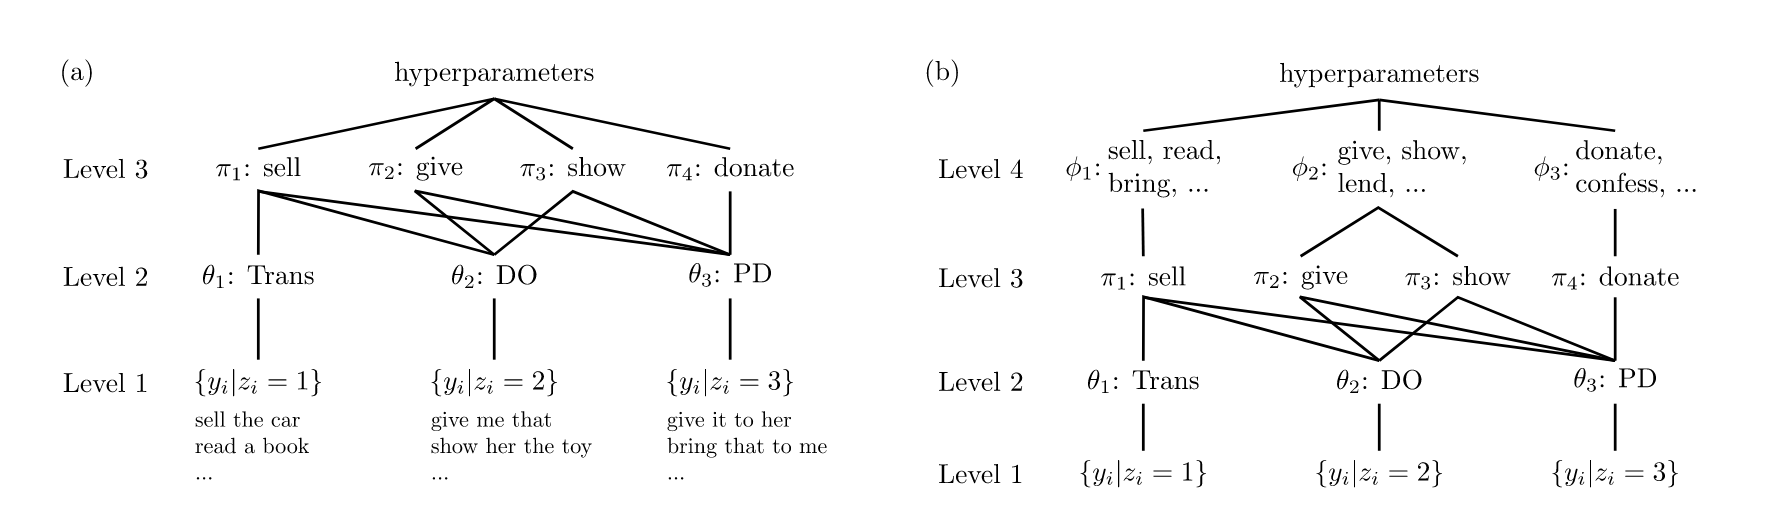
\includegraphics[width=\textwidth]{figures/verb_alternation_classes.png}
    \centering    
\end{figure}

Approach similar to \citet{parisien2010}, where a Hierarchical Dirichlet process is extended to account for diathesis alternations. Each verb will be represented by its distribution over the valency frames of the language, which are then clustered in a similar process as step 2.


\subsection{Cross-lingual verb sense alignment}\label{subsec:verblist}

A cross-lingual aligned list of counterpart verbs will be needed to compare the verb classes and valency frames. The easiest way to do this is likely through existing cross-lingual word lists such as LanguageNet, part of the PanLex project. http://uakari.ling.washington.edu/languagenet/available/

Alternatively, lexicon induction from cross-lingual word embeddings and other NLP methods may also be considered.

\subsection{Information theory}\label{subsec:infotheory}

Complexity and point-wise mutual information, like in \citet{say2014}.
Complexity measure:

Point-wise mutual information (PMI)